% \begin{center}
% \begin{minipage}{0.6\textwidth}
% \textit{\Large Talent is uniformly distributed. Opportunity is not}\footnote{\html{https://trademarks.justia.com/870/43/talent-is-equally-distributed-globally-but-opportunity-is-87043434.html}{Trademark}}.\\

% \hfill --- Jessy Grizzle, University of Michigan Robotics, August 2020
% \end{minipage}

% \end{center}


\hfill \textit{\Large Talent is uniformly distributed. Opportunity is not.}\footnote{\href{https://trademarks.justia.com/870/43/talent-is-equally-distributed-globally-but-opportunity-is-87043434.html}{Trademark}}\\

\hfill Jessy Grizzle, University of Michigan Robotics, August 2020


\bigskip

The Robotics faculty seek to prepare students for the era of Information, AI, Data, and, of course, Robotics. To accomplish this, we must leave behind the Sputnik-inspired means of educating engineers, where we put our students through four semesters of Calculus before they are able to engage with any exciting engineering problems. We are replacing the standard approach with the idea that all aspects of the theory of mathematics should be brought alive through computation and compelling case studies. We are combining math education with modern computational tools and replacing most exams with accomplishment-based assessments through projects based on real engineering examples.

This book covers the essence of integral and differential Calculus of single variable functions, Jacobians and gradients of multivariable functions, and enough material on ordinary differential equations to understand the existence and uniqueness of solutions and how to compute solutions numerically. To bring the material to life, the course takes the design of a stabilizing feedback controller for the BallBot used in \textbf{ROB 311 Build Robots and Make them Move}\footnote{The course was designed 
 by Prof. Elliott Rouse and piloted in Fall 2022 with the assistance of PhD student Yves Nazon and Engineer  Senthur Raj Ayyappan. \textbf{Image credit: Senthur Raj Ayyappan, Summer 2023}.} as an end goal. Along the way, we'll develop tools for understanding a dynamic model of the BallBot.
    
    \begin{center}
    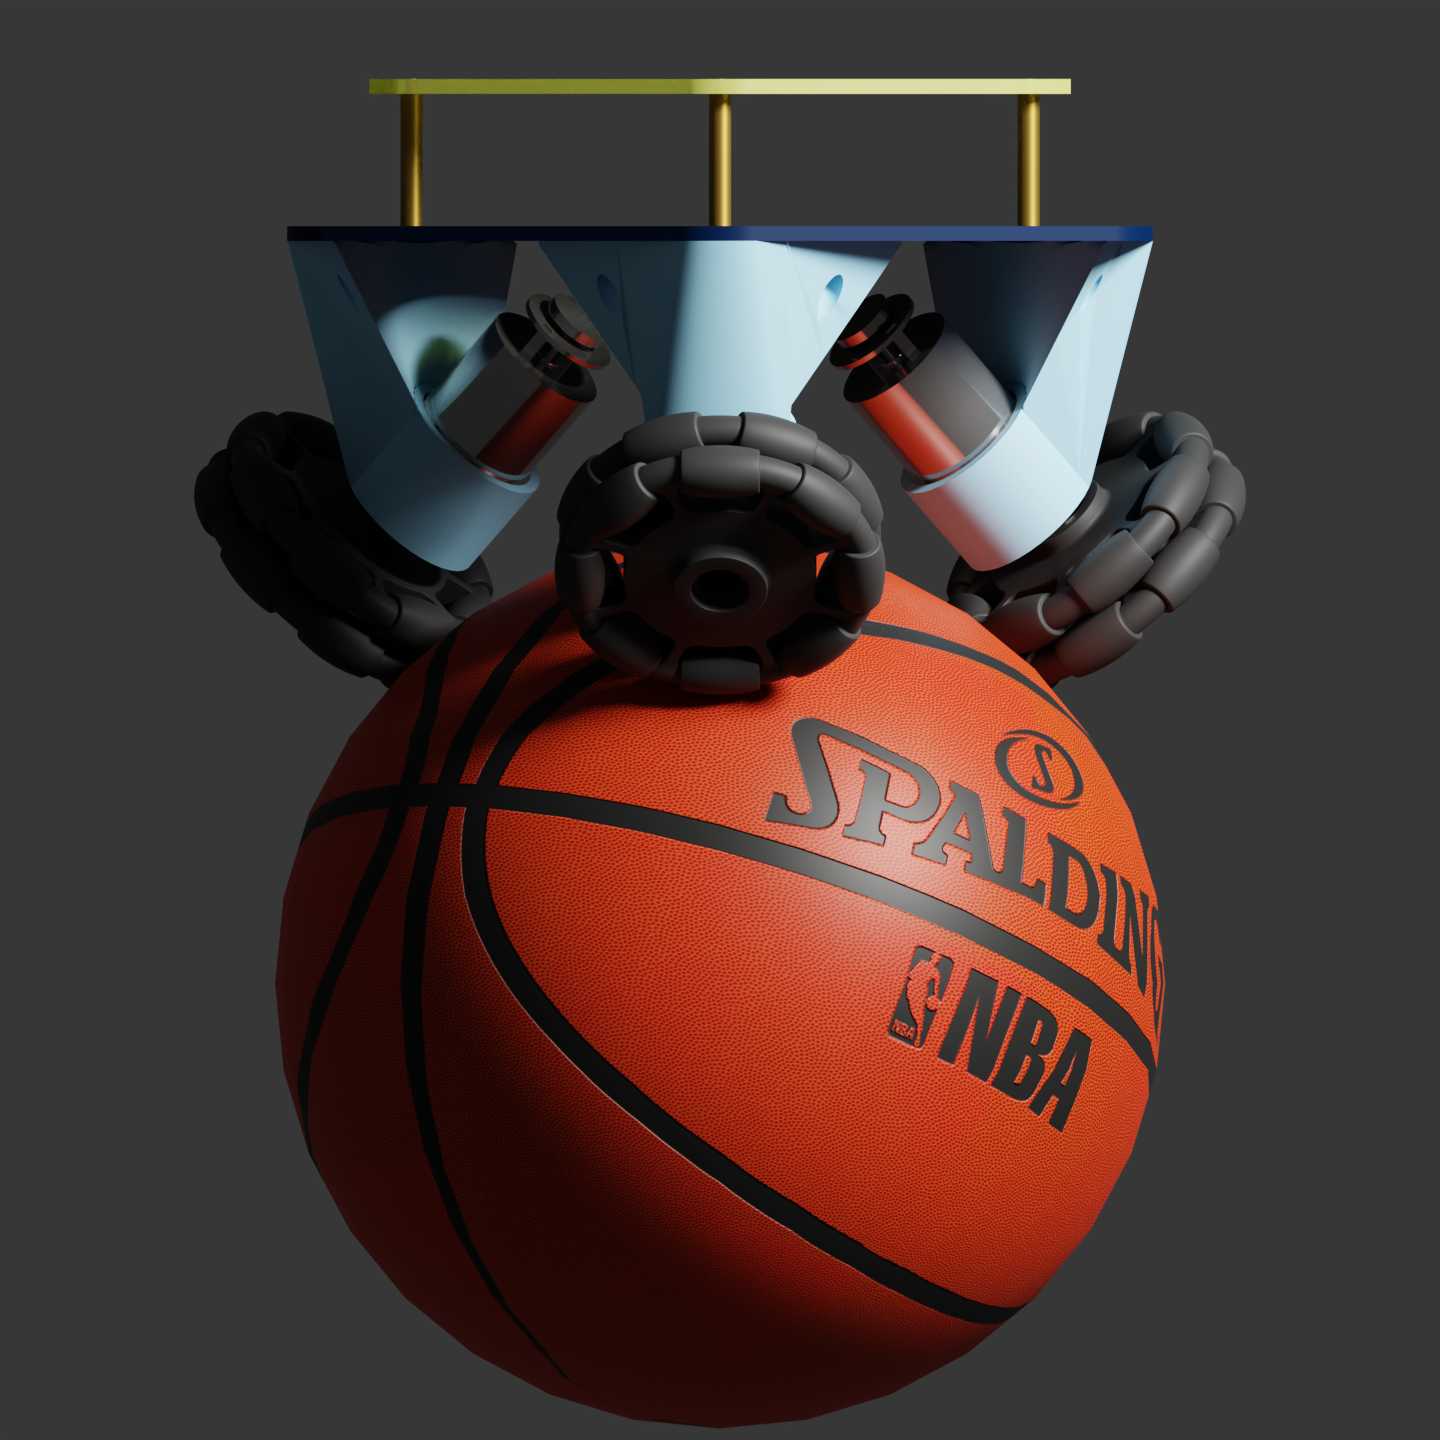
\includegraphics[width=0.5\columnwidth]{graphics/CoverPrefacePhilosophy/ballbot.png}
    \end{center}

This book treats the following topics:
\begin{itemize}
    \item A pre-Calculus review with an emphasis on careful statements of the key results, with correct notation. Special attention is given to topics where students often struggle, such as domains, codomains, and ranges of functions, inverse functions, logarithms, and the Binomial Theorem. A multi-link robot manipulator is introduced, and its forward kinematics are computed using standard trigonometry. Euler's Formula is included early on due to its importance in understanding solutions of differential equations later in the textbook. The majority of this material is meant for self-study. 
    \item As part of the pre-Calculus review, the dread that many students bring with them into a Calculus course is acknowledged, along with resources for confidence building. 
    \item The Approximation Principle, or how to compute quantities with lower and upper bounds on their accuracy. This introduces the spirit of Calculus before the conceptual hurdles of integration and differentiation.
    \item The spirit of Calculus is furthered through a discussion of why mathematicians use proofs: simply put, what often seems obviously wrong or correct might be neither! Cantor's discovery of uncountable sets and his repudiation by the mathematical community of his day is used as a cautionary tale, treated at an appropriate level for Y2 students. The most used proof technique in the book, induction, is covered with application to finite sums that appear in integration. Importantly, these sums are rational functions of the number of terms in the sum. Next, the problem of approximating the area under curves is broached and solved for monomials before ever talking about limits or integration. A first introduction to limits is done in the context of rational functions, where the supporting arguments can be made transparent and where important motivating examples are already at hand from the discussion of the area under monomials. This will lessen the resistance to limits when they are done correctly in a later chapter in the context of continuous functions.
    \item Definite Integrals for functions of a single variable from fundamental and numerical perspectives, with application to:
    \begin{itemize}
        \item determining a robot's path from knowledge of its speed or velocity, 
        \item ballistic motion,
        \item area between two functions, with this topic applied to determining important parameters for building planar dynamical models of robots, such as total mass, center of mass, and moment of inertia.
    \end{itemize}
    \item Limits are a workhorse of Calculus. And while students often dislike them, especially the epsilon-delta definitions, there is no getting around their centrality to really understanding how Calculus works. Consequently, limits are explored from both fundamental and computational perspectives. Limits are then applied to the fundamentals of Calculus itself, through the study of continuous functions showing the power of taking limits inside of continuous functions. Other key topics of a rather technical nature, such as the existence of minima and maxima find their place with this material.
    \item Derivatives of functions of a single variable and several variables, with emphasis on how to compute derivatives of complicated functions using modern software tools. For a practicing engineer, there is no drudgery involved with computing derivatives and students of the course understand why that is so.
    \item The applications of derivatives are so important and numerous that they are assembled into a separate chapter. Topics include,
        \begin{itemize}
        \item root finding for scalar and vector functions, along with appropriate software tools,
        \item gradient descent, along with appropriate software tools,
        \item minimization with equality constraints, along with appropriate software tools, with application to reaching into a highly constrained space with a manipulator,
        \item determining a robot's speed from knowledge of its trajectory, 
        \item two important quantities for building dynamical models of robots, namely, kinetic energy and potential energy, and 
        \item combining them to form the Lagrangian of a planar mechanical system comprised of rigid bodies,
        \item Lagrange's method is introduced as a source of the robot equations! 
    \end{itemize}
    \item Antiderivatives and the two Fundamental Theorems of Calculus, with emphasis on modern software tools for doing the computations. In most Calc II courses, antiderivatives are taught as the primary way to do integration, which is a huge disservice to STEM students, who, outside of a College Campus, will never have a sufficiently simple integrand to which any of the standard methods for antiderivatives apply. Hence, antiderivatives are placed in a more realistic context of being able to understand simple intergrals very rapidly and to provide insight, with numerical tools being the real workhorse in practice. ChatGPT and the Wolfram plugin are highlighted as the modern equivalent of the ``Handbook of Mathematical Functions with Formulas, Graphs, and Mathematical Tables,'' which we all used back in the day. 
    \item By the time Ordinary Differential Equations or ODEs roll around, examples of ODEs have occurred on three different occasions. Hence, the question is not so much what is an ODE, but how does one solve an ODE and how are ODEs used in real life case studies. One-dimensional ODEs from drag chutes and parachutes are introduced and then solved via separation of variables, until literally, a one-dimensional quadratic drag model is treated for which no closed-form solution is known. This motivates numerical solvers, which also treat high-dimendional problems for which all of the traditional methods taught in an ODE course fail. The existence and uniqueness of solutions are addressed and applied to small- and medium-sized models of systems. An intensive study of linear systems of ODEs is done, drawing on the students' background in linear algebra. The matrix exponential is analyzed, and conditions for exponential stability of an equilibrium are presented, drawing upon prior experience with eigenvalues and eigenvalues (after appropriate reminders). Jacobian linearizations of nonlinear ODEs provide a rich source of real-life examples.
    \item A very targeted introduction to the Laplace Transform is given, with the goal of understanding poles and zeros of transfer functions, and how PD controllers work. The main application treated in the chapter is the stabilization of a Segway mobile robot, which sets students up for their final project, designing a feedback controller for a simulation model of the BallBot. 
    \item A broader introduction to linear feedback control is provided in an Appendix. 
\end{itemize} 

That's a lot for one semester; hence, we've had to be careful about what we cover versus omit so as to provide the learner with an expedited understanding of Calculus and how to apply it. To be clear, the course does not seek to replace the full four semesters of Calculus. To round out our Michigan students' mathematical education, we will require them to take two additional Math courses from a \hyperlink{CuratedListCourses}{\textcolor{red}{\bf carefully curated list}}. Hopefully, many students will be inspired to take Math 215 Multivariable and Vector Calculus and proof-based courses such as, Math 217 Linear Algebra, where, already knowing quite a bit about linear algebra through ROB 101, they can focus on learning how proofs work, or Math 451 Advanced Calculus I, a proof-based version of Calculus taught through the lens of Real Analysis in $\real^n$.

\textbf{Caveat:} While we believe this book will prepare students uncommonly well for real engineering, you, the student, still must succeed in your Engineering courses, most of which will assume you learned Calculus in the standard manner. You'll have to compute derivatives and integrals on timed, written exams in those classes without access to modern software tools. In this textbook, we do our best to prepare you for this as well. Until our teaching philosophy is more widely adopted in Engineering, you must learn how to perform certain methods by hand in order to obtain your BS Degree in Engineering. We'll highlight some of that material in our lectures. Your ultimate source for the Calculus techniques you must know how to complete by hand will be the lectures and HW problems in your Engineering courses themselves. We are confident that the material in this book will provide an excellent reference throughout your undergraduate education.\\

\textbf{Jessy Grizzle}\\
Ann Arbor, Michigan USA, August 2024